% Options for packages loaded elsewhere
\PassOptionsToPackage{unicode}{hyperref}
\PassOptionsToPackage{hyphens}{url}
%
\DocumentMetadata{
 lang=en,
 pdfversion=2.0,
 pdfstandard=ua-2,
 pdfstandard=a-4,
 testphase=latest
 }
\documentclass[
]{article}
\usepackage{amsmath,amssymb}
\usepackage{iftex}
\ifPDFTeX
  \usepackage[T1]{fontenc}
  \usepackage[utf8]{inputenc}
  \usepackage{textcomp} % provide euro and other symbols
\else % if luatex or xetex
  \usepackage{unicode-math} % this also loads fontspec
  \defaultfontfeatures{Scale=MatchLowercase}
  \defaultfontfeatures[\rmfamily]{Ligatures=TeX,Scale=1}
\fi
\usepackage{lmodern}
\ifPDFTeX\else
  % xetex/luatex font selection
\fi
% Use upquote if available, for straight quotes in verbatim environments
\IfFileExists{upquote.sty}{\usepackage{upquote}}{}
\IfFileExists{microtype.sty}{% use microtype if available
  \usepackage[]{microtype}
  \UseMicrotypeSet[protrusion]{basicmath} % disable protrusion for tt fonts
}{}
\makeatletter
\@ifundefined{KOMAClassName}{% if non-KOMA class
  \IfFileExists{parskip.sty}{%
    \usepackage{parskip}
  }{% else
    \setlength{\parindent}{0pt}
    \setlength{\parskip}{6pt plus 2pt minus 1pt}}
}{% if KOMA class
  \KOMAoptions{parskip=half}}
\makeatother
\usepackage{xcolor}
\usepackage[margin=1in]{geometry}
\usepackage{color}
\usepackage{fancyvrb}
\newcommand{\VerbBar}{|}
\newcommand{\VERB}{\Verb[commandchars=\\\{\}]}
\DefineVerbatimEnvironment{Highlighting}{Verbatim}{commandchars=\\\{\}}
% Add ',fontsize=\small' for more characters per line
\usepackage{framed}
\definecolor{shadecolor}{RGB}{248,248,248}
\newenvironment{Shaded}{\begin{snugshade}}{\end{snugshade}}
\newcommand{\AlertTok}[1]{\textcolor[rgb]{0.94,0.16,0.16}{#1}}
\newcommand{\AnnotationTok}[1]{\textcolor[rgb]{0.56,0.35,0.01}{\textbf{\textit{#1}}}}
\newcommand{\AttributeTok}[1]{\textcolor[rgb]{0.13,0.29,0.53}{#1}}
\newcommand{\BaseNTok}[1]{\textcolor[rgb]{0.00,0.00,0.81}{#1}}
\newcommand{\BuiltInTok}[1]{#1}
\newcommand{\CharTok}[1]{\textcolor[rgb]{0.31,0.60,0.02}{#1}}
\newcommand{\CommentTok}[1]{\textcolor[rgb]{0.56,0.35,0.01}{\textit{#1}}}
\newcommand{\CommentVarTok}[1]{\textcolor[rgb]{0.56,0.35,0.01}{\textbf{\textit{#1}}}}
\newcommand{\ConstantTok}[1]{\textcolor[rgb]{0.56,0.35,0.01}{#1}}
\newcommand{\ControlFlowTok}[1]{\textcolor[rgb]{0.13,0.29,0.53}{\textbf{#1}}}
\newcommand{\DataTypeTok}[1]{\textcolor[rgb]{0.13,0.29,0.53}{#1}}
\newcommand{\DecValTok}[1]{\textcolor[rgb]{0.00,0.00,0.81}{#1}}
\newcommand{\DocumentationTok}[1]{\textcolor[rgb]{0.56,0.35,0.01}{\textbf{\textit{#1}}}}
\newcommand{\ErrorTok}[1]{\textcolor[rgb]{0.64,0.00,0.00}{\textbf{#1}}}
\newcommand{\ExtensionTok}[1]{#1}
\newcommand{\FloatTok}[1]{\textcolor[rgb]{0.00,0.00,0.81}{#1}}
\newcommand{\FunctionTok}[1]{\textcolor[rgb]{0.13,0.29,0.53}{\textbf{#1}}}
\newcommand{\ImportTok}[1]{#1}
\newcommand{\InformationTok}[1]{\textcolor[rgb]{0.56,0.35,0.01}{\textbf{\textit{#1}}}}
\newcommand{\KeywordTok}[1]{\textcolor[rgb]{0.13,0.29,0.53}{\textbf{#1}}}
\newcommand{\NormalTok}[1]{#1}
\newcommand{\OperatorTok}[1]{\textcolor[rgb]{0.81,0.36,0.00}{\textbf{#1}}}
\newcommand{\OtherTok}[1]{\textcolor[rgb]{0.56,0.35,0.01}{#1}}
\newcommand{\PreprocessorTok}[1]{\textcolor[rgb]{0.56,0.35,0.01}{\textit{#1}}}
\newcommand{\RegionMarkerTok}[1]{#1}
\newcommand{\SpecialCharTok}[1]{\textcolor[rgb]{0.81,0.36,0.00}{\textbf{#1}}}
\newcommand{\SpecialStringTok}[1]{\textcolor[rgb]{0.31,0.60,0.02}{#1}}
\newcommand{\StringTok}[1]{\textcolor[rgb]{0.31,0.60,0.02}{#1}}
\newcommand{\VariableTok}[1]{\textcolor[rgb]{0.00,0.00,0.00}{#1}}
\newcommand{\VerbatimStringTok}[1]{\textcolor[rgb]{0.31,0.60,0.02}{#1}}
\newcommand{\WarningTok}[1]{\textcolor[rgb]{0.56,0.35,0.01}{\textbf{\textit{#1}}}}
\usepackage{graphicx}
\makeatletter
\def\maxwidth{\ifdim\Gin@nat@width>\linewidth\linewidth\else\Gin@nat@width\fi}
\def\maxheight{\ifdim\Gin@nat@height>\textheight\textheight\else\Gin@nat@height\fi}
\makeatother
% Scale images if necessary, so that they will not overflow the page
% margins by default, and it is still possible to overwrite the defaults
% using explicit options in \includegraphics[width, height, ...]{}
\setkeys{Gin}{width=\maxwidth,height=\maxheight,keepaspectratio}
% Set default figure placement to htbp
\makeatletter
\def\fps@figure{htbp}
\makeatother
\setlength{\emergencystretch}{3em} % prevent overfull lines
\providecommand{\tightlist}{%
  \setlength{\itemsep}{0pt}\setlength{\parskip}{0pt}}
\setcounter{secnumdepth}{-\maxdimen} % remove section numbering
\ifLuaTeX
  \usepackage{selnolig}  % disable illegal ligatures
\fi
\usepackage{bookmark}
\IfFileExists{xurl.sty}{\usepackage{xurl}}{} % add URL line breaks if available
\urlstyle{same}
\hypersetup{
  pdftitle={Create an accessible pdf from rmarkdown with alt tags only},
  hidelinks,
  pdfcreator={LaTeX via pandoc}}

\title{Create an accessible pdf from rmarkdown with alt tags only}
\author{}
\date{\vspace{-2.5em}}

\begin{document}
\maketitle

\subsection{Table of contents}\label{table-of-contents}

\begin{itemize}
\tightlist
\item
  \hyperref[who-is-this-document-for]{Who is this document for?}
\item
  \hyperref[steps-in-process]{Step in process}
\item
  \hyperref[testing-figure-sizes]{Testing figure sizes}
\end{itemize}

\subsection{Who is this document for?}\label{who-is-this-document-for}

This document is for people who prefer to use flavors of markdown for
their document writing instead of Microsoft Word. When writing in
markdown issues arise when converting to pdf. In particular alt text for
images are not displayed or transferred resulting in pdfs failing to
pass accessibility checks.

\subsection{Prerequisites}\label{prerequisites}

Please make sure that you update the \texttt{tinytex} package. You will
need to install a bundle that is different from the default bundle.

\begin{Shaded}
\begin{Highlighting}[]
\NormalTok{tinytex}\SpecialCharTok{::}\FunctionTok{install\_tinytex}\NormalTok{(}\AttributeTok{bundle =} \StringTok{"TinyTex{-}2"}\NormalTok{)}
\end{Highlighting}
\end{Shaded}

For this particular example you will need to install the
\href{https://github.com/NOAA-EDAB/ecodata}{\texttt{ecodata}} package.

\subsection{Steps in process}\label{steps-in-process}

\begin{itemize}
\tightlist
\item
  Knit the Rmd file
\item
  Edit the \texttt{tex} file created
\item
  Add the following code to the \texttt{tex} file right above the line
  \texttt{\textbackslash{}documentclass\{article\}}
\end{itemize}

\begin{verbatim}
\DocumentMetadata{
 lang=en,
 pdfversion=2.0,
 pdfstandard=ua-2,
 pdfstandard=a-4,
 testphase=latest
 }
\end{verbatim}

\begin{itemize}
\tightlist
\item
  Save and compile this \texttt{tex} file by clicking the ``Compile
  PDF'' button in RStudio
\item
  open pdf and perform a \texttt{full\ check} (found in the
  accessibility tab)
\end{itemize}

\subsection{Testing figure sizes}\label{testing-figure-sizes}

All images were created with a resolution of 96 dpi.

Each figure has different number of horizontal and vertical pixels.

\textbf{Note: the figure caption will be the name of the image file path
for png included using \texttt{knitr}}

\subsubsection{Include a file}\label{include-a-file}

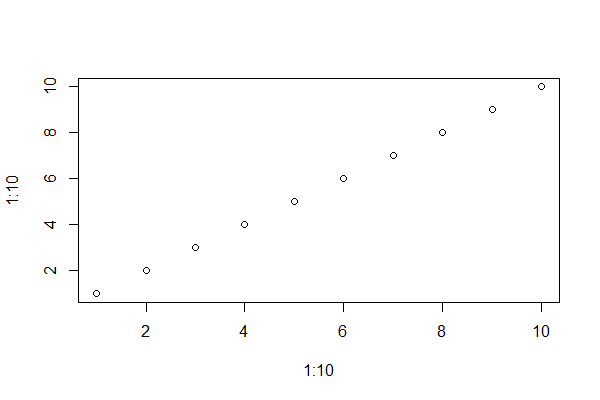
\includegraphics[width=600px]{figures/test6}

\subsubsection{Create an image from a code
chunk}\label{create-an-image-from-a-code-chunk}

\includegraphics[width=600px]{example3_files/figure-latex/ecodata-gsi-1}

\subsubsection{Create an image from a code chunk with no width
specified}\label{create-an-image-from-a-code-chunk-with-no-width-specified}

\includegraphics{example3_files/figure-latex/ecodata-blue-runner-1}

\end{document}
